\section{Substrate ``Anchor'' Sites for Continuous Thin Film Morphology}
\label{Chap:Ag/ZnO:section:anchor}

As we mentioned before, random surface defects may have a positive effect on forming a continuous thin film. This may come from strong interactions between surface defect sites and Ag atoms. In this section, we will investigate the possibility of using the surface ``anchor'' site to improve the thin film continuity. A similar idea was initially proposed by Chambers et al. \cite{chambers2002laminar}. They considered the situation of transition metal getting oxidized and immobilized by the ZnO substrate. This is true when experiments are done in \ac{UHV}. But sputtering, especially industry-level sputtering usually happens in \ac{HV} conditions and the main source of oxygen is the residual gas which consists of water vapor as majorities as pointed out by Anders et al. \cite{anders2006smoothing} in 2006. In this section, a new criterion is proposed to search for stable anchor sites that can stand with water vapor and $\text{H}_{\text{2}}$ attacks.

Therefore, we propose three criteria that are important for surface anchor elements: i) they can survive the attacks of water vapor($\text{H}_{\text{2}}\text{O}$) and $\text{H}_{\text{2}}$; ii) they have high diffusion barriers on saturated ZnO substrates; iii) they have strong bonding strength with Ag atoms.

For the first criterion, four different reactions are considered. The first two correspond to the two possible water ($\text{H}_{\text{2}}\text{O}$) dissociation reactions on the ZnO substrate with one ``anchor'' site, as shown in Figure \ref{Chap:Ag/ZnO:fig:12a}. The upper reaction represents an incoming water molecule dissolve to one OH group attached to the ``anchor'' site and one H atom at a remote ``anchor'' site. The lower plot of Figure \ref{Chap:Ag/ZnO:fig:12a}, represents the reaction of an incoming water molecule dissolve to one OH group attached to the ``anchor'' site and one H atom at a nearby O atom top. The third and fourth reaction corresponds to the two possible $\text{H}_{\text{2}}$ dissociation reactions on the ZnO substrate with one ``anchor'' site, as shown in Figure \ref{Chap:Ag/ZnO:fig:12a}. We summarize the 4 reactions as below:
\begin{subequations}
\begin{align}
H_2O + 2 ZnO-X & \rightarrow ZnO-X-OH + ZnO-X-H
 \label{Chap:Ag/ZnO:eq:anchor1}\\
H_2O + ZnO-X & \rightarrow H-ZnO-X-OH
 \label{Chap:Ag/ZnO:eq:anchor2}\\
H_2 + 2 ZnO-X & \rightarrow ZnO-X-H + ZnO-X-H
 \label{Chap:Ag/ZnO:eq:anchor3}\\
H_2 + ZnO-X & \rightarrow H-ZnO-X-H
 \label{Chap:Ag/ZnO:eq:anchor4}
\end{align}
\end{subequations}


\newpage
\begingroup
\begin{figure}[!ht]
  \centering
  \subfigure[]{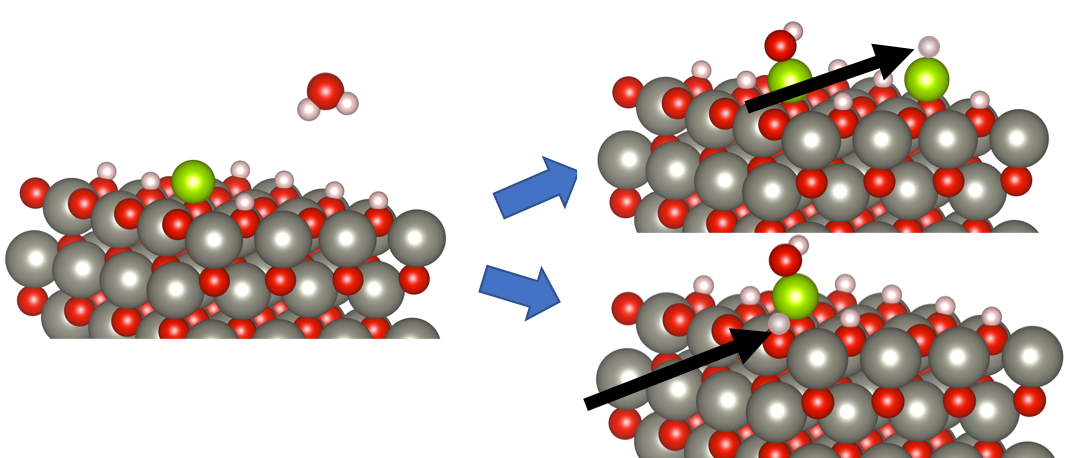
\includegraphics[width=0.85\linewidth]{Chap4/plots/Picture12a.png}}\label{Chap:Ag/ZnO:fig:12a}
  \subfigure[]{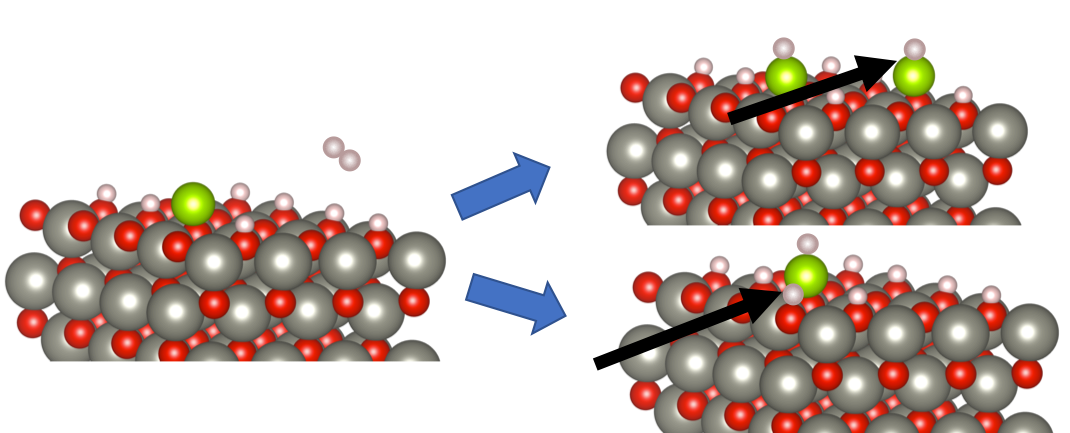
\includegraphics[width=0.85\linewidth]{Chap4/plots/Picture12b.png}}\label{Chap:Ag/ZnO:fig:12b}
\caption[Possible water and $\text{H}_{\text{2}}$ dissociation reactions on ZnO substrate with ``anchor'' sites.]{Possible water and $\text{H}_{\text{2}}$ dissociation reactions on ZnO substrate with one ``anchor'' site. (a) Two possible water ($\text{H}_{\text{2}}\text{O}$) dissociation reactions on ZnO substrate with anchor sites. (b) Two possible $\text{H}_{\text{2}}$ dissociation reactions on ZnO substrate with anchor sites. Red and grey atoms are O and Zn atoms, respectively. Green atoms represent the ``anchor'' element on ZnO substrate surfaces. Pink ones are H atoms.}
\label{Chap:Ag/ZnO:fig12}
\end{figure}
\endgroup

In order to have the ``anchor'' elements staying reactive on ZnO substrates, all the four equations need to yield positive enthalpies. After screening the first criterion, as shown in Figure \ref{Chap:Ag/ZnO:fig13}, Pd, Sb, Se, Sn, Cd, and Te can survive the environment of water and H. Cd is eliminated as it is an extremely toxic industrial and environmental pollutant.

\begingroup
\begin{figure}[!ht]
  \centering
  \subfigure[]{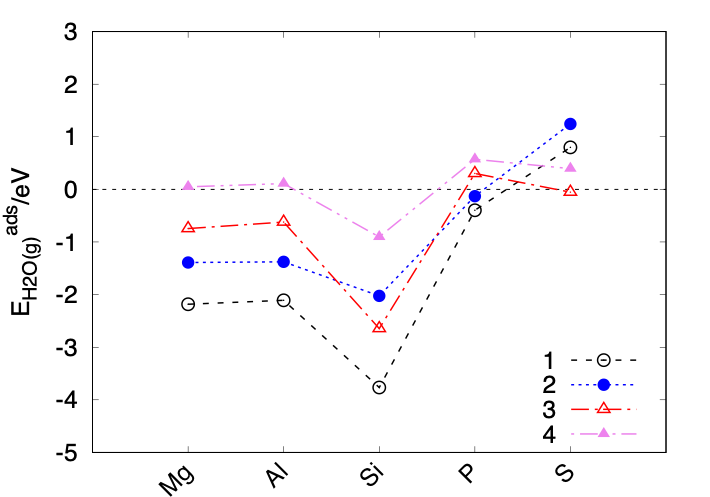
\includegraphics[width=0.49\linewidth]{Chap4/plots/Picture13a.png}}\label{Chap:Ag/ZnO:fig:13a}
  \subfigure[]{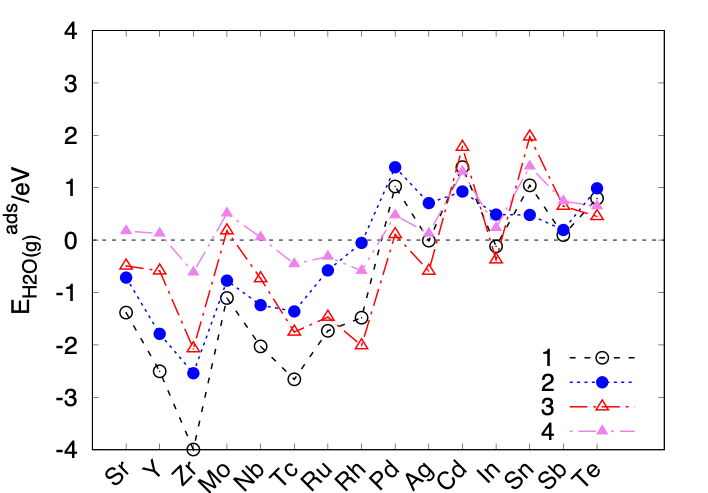
\includegraphics[width=0.49\linewidth]{Chap4/plots/Picture13b.png}}\label{Chap:Ag/ZnO:fig:13b}
  \\
  \subfigure[]{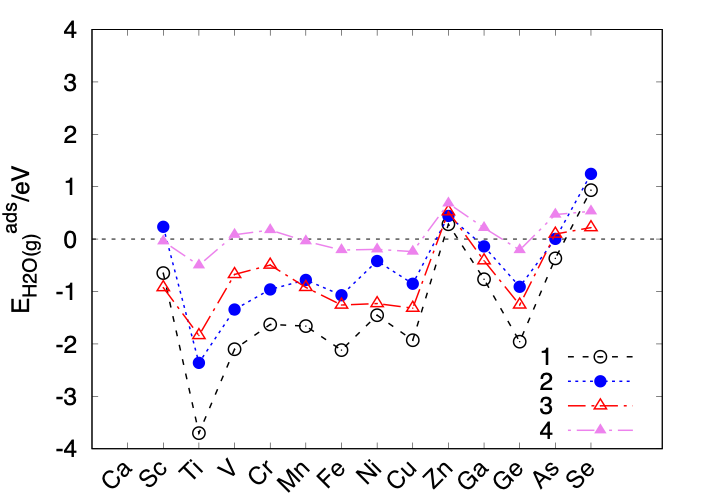
\includegraphics[width=0.49\linewidth]{Chap4/plots/Picture13c.png}}\label{Chap:Ag/ZnO:fig:13c}
  \subfigure[]{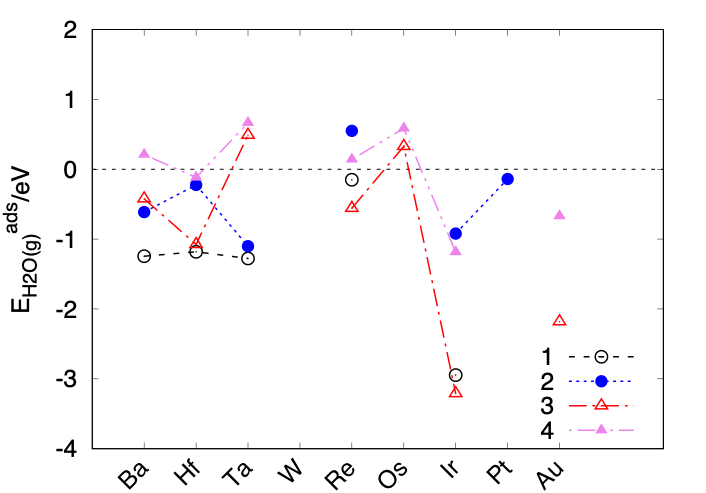
\includegraphics[width=0.49\linewidth]{Chap4/plots/Picture13d.png}}\label{Chap:Ag/ZnO:fig:13d}
\caption[Water and $\text{H}_{\text{2}}$ dissociation reactions energies on ZnO substrate with ``anchor'' sites.]{Water and $\text{H}_{\text{2}}$ dissociation reactions energies on ZnO substrate with ``anchor'' sites. Reaction 1 and 2 corresponds to 2 possible water dissociation reactions in Figure
\ref{Chap:Ag/ZnO:fig12} (a), respectively. Reaction 3 and 4 corresponds to 2 possible $\text{H}_{\text{2}}$ dissociation reactions in Figure \ref{Chap:Ag/ZnO:fig12} (b), respectively.}
\label{Chap:Ag/ZnO:fig13}
\end{figure}
\endgroup

\begin{table}[!ht]
\caption[``Anchor'' elements diffusion barriers on ZnO saturated with $\frac{1}{2}$ \ac{ML} H.]{``Anchor'' elements diffusion barriers on ZnO saturated with $\frac{1}{2}$ \ac{ML} H.}
\label{Chap:Ag/ZnO:tab1}
\centering
\begin{tabular}{cc}
\\
\hline
\hline
Substrate & \begin{tabular}[c]{@{}c@{}}Diffusion barrier on ZnO saturated\\ with $\frac{1}{2}$ \ac{ML} H [eV]\end{tabular} \\ \hline
Ag        & 0.077                                                                                                          \\
Pd        & 0.275                                                                                                          \\
Sb        & 0.111                                                                                                          \\
Se        & 1.338                                                                                                          \\
Sn        & 0.341                                                                                                          \\
Te        & 0.999                                                                                                          \\ \hline
\hline
\end{tabular}
\end{table}

For the second and third criteria, all the 5 elements have orders of magnitude higher diffusion barriers compared to Ag atoms on fully-saturated ZnO substrates, as shown in Table \ref{Chap:Ag/ZnO:tab1}. Moreover, as we can see from Table \ref{Chap:Ag/ZnO:tab2}, all the 5 elements have much stronger bonding strengths to an Ag atom compared to bare ZnO substrates as well.

\begin{table}[!ht]
\caption[Ag adsorption on saturated ZnO substrate with ``anchor'' sites.]{Ag adsorption on saturated ZnO substrate with ``anchor'' sites.}
\label{Chap:Ag/ZnO:tab2}
\centering
\begin{tabular}{cc}
\\
\hline
\hline
Substrate              & Adsorption energy(eV) \\ \hline
ZnO with $\frac{1}{2}$ \ac{ML}    & -0.716                \\
Pd & -1.716                \\
Sb & -2.242                \\
Se & -2.055                \\
Sn & -2.284                \\
Te & -1.931                \\ \hline
\hline
\end{tabular}
\end{table}

In order to demonstrate the effect of surface ``anchor'' sites on Ag thin film morphology, \ac{GCMC} simulations are conducted. 0.05\ac{ML} of substrate atoms are randomly changed to ``anchor'' site atoms which has a stronger binding to Ag. Then 10\ac{ML} of Ag atoms are deposited. In Figure \ref{Chap:Ag/ZnO:fig14}, a much more continuous Ag thin film can be seen with 0.05\ac{ML} of ``anchor'' sites. With randomly distributed ``anchor'' sites, more nuclei can be achieved, hence more continuous ultra-thin film. The number of anchor sites added on ZnO substrates is limited, so there will not be a great change of Ag/ZnO interfacial energies globally. But the anchor sites might increase the interfacial energies locally. And the mechanisms of anchor sites to increase Ag wettability are from two aspects: 1) increasing adsorption energies of individual Ag atoms on ZnO saturated surfaces; 2) increase Ag surface diffusion barriers.

\newpage
\begingroup
\begin{figure}[!ht]
  \centering
  \subfigure[]{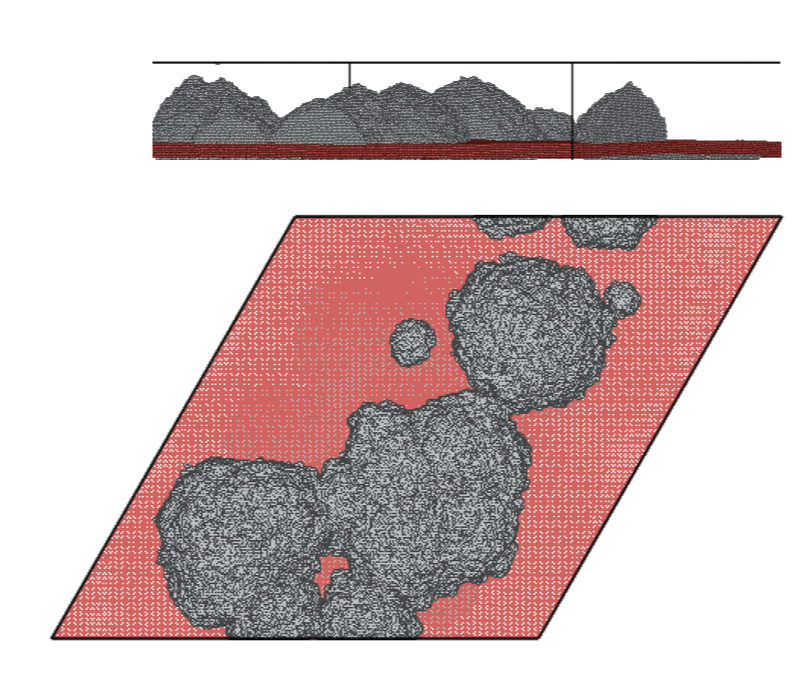
\includegraphics[width=0.65\linewidth]{Chap4/plots/Picture14a.png}}\label{Chap:Ag/ZnO:fig:14a}
  \subfigure[]{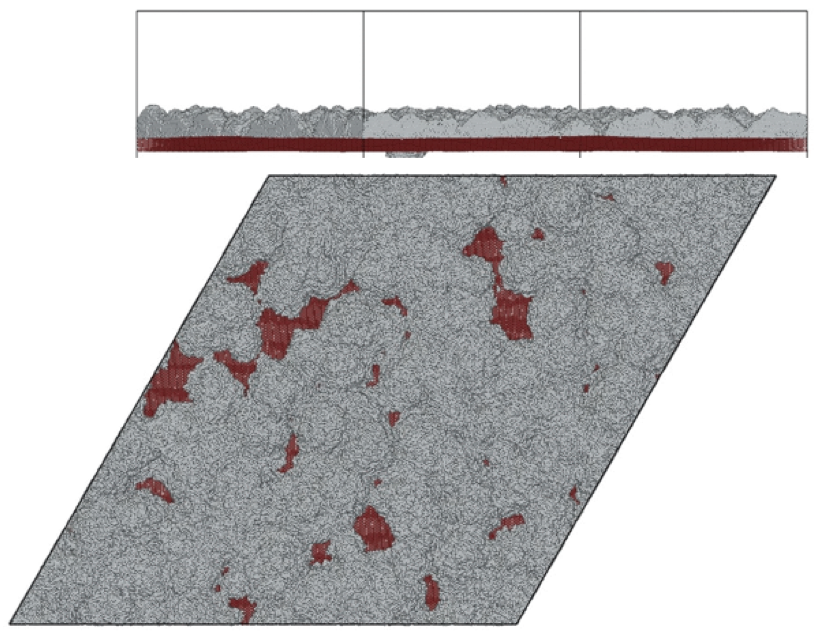
\includegraphics[width=0.65\linewidth]{Chap4/plots/Picture14b.png}}\label{Chap:Ag/ZnO:fig:14b}
\caption[GCMC simulation results for 10\ac{ML} Ag deposition on ZnO with and without 0.05\ac{ML} surface ``anchor'' sites.]{\ac{GCMC} simulation results for 10\ac{ML} Ag deposition on ZnO with and without 0.05\ac{ML} surface ``anchor'' sites. (a) Ag island growth pattern on ZnO without surface ``anchor'' sites. (b) Ag island growth pattern on ZnO with 0.05\ac{ML} surface ``anchor'' sites.}
\label{Chap:Ag/ZnO:fig14}
\end{figure}
\endgroup